\documentclass{article}

\usepackage{graphicx}
\usepackage{subfigure}
\usepackage[hypcap]{caption}
\usepackage{listings}

\title{Experimental Design and Data Analysis: Assignment 2}
\author{Andrew Bedard \& Simone van Gompel(2567525) \\ Group 19}

\begin{document}

  \maketitle

  \section{Exercise 1}
    Exercise 1 stuff...

  \section{Exercise 2}
    I needed to put the light1882 on 1 line, else it can't be imported as a table,
    because it would not have a full last line.
    See Fig:\ref{fig:HistEx2} for the histograms of the two datasets.\\
    The 95\% confidence interval of the mean of Light1879 is 836.7226 - 868.0774\\
    The 95\% confidence interval of the mean of Light1879 is 712.4417 - 799.9931\\
    The 95\% confidence interval of the median of Light1879 is 834.5142 - 865.4858\\
    The 95\% confidence interval of the median of Light1879 is 730.2243 - 817.7757\\

    \begin{figure}
      \subfigure[1879]
      {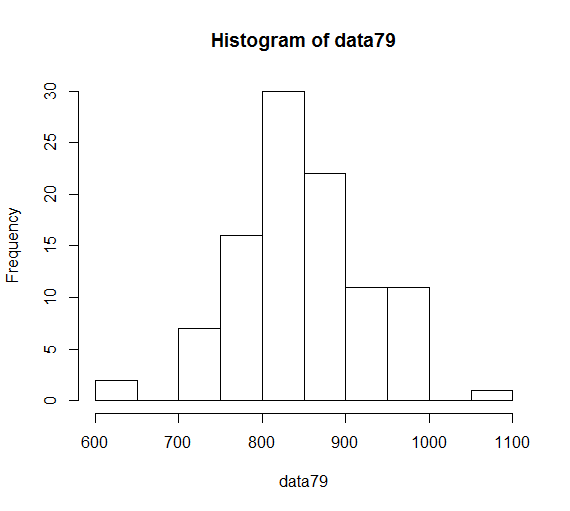
\includegraphics[scale=0.35]{../results/Hist1879.png} }
      \subfigure[1882]
      {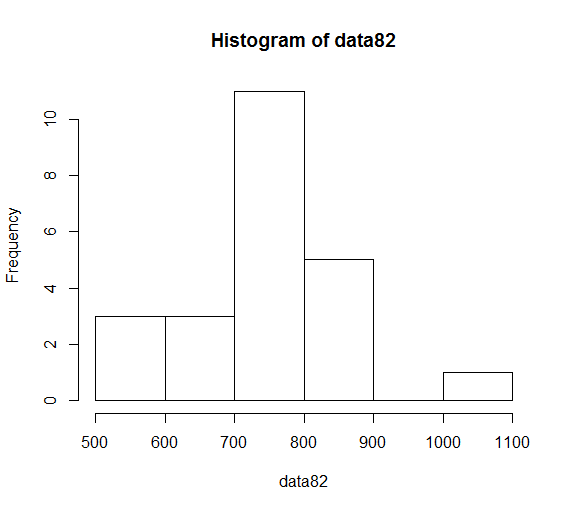
\includegraphics[scale=0.35]{../results/Hist1882.png} }
      \caption{Histograms of the datasets Light1879 and Light1882}
      \label{fig:HistEx2}
    \end{figure}

  \section{Exercise 3}
    Looking at the graphs of the data, see Fig:\ref{fig:GraphKLM} , it is clear that this dataset is not normally distributed.
    So the t-test should not be used.
    Instead of this, we use the sign-test, which can be used for any other sort of distribution.
    The results of this test are as follows:\\
    \begin{lstlisting}[language=R]
        One-sample Sign-Test

      data:  klm
      s = 36, p-value = 0.155
      alternative hypothesis: true median is not equal to 35
      95 percent confidence interval:
       32.00000 56.07713
      sample estimates:
      median of x 
               42 

                        Conf.Level L.E.pt  U.E.pt
      Lower Achieved CI     0.9481     32 56.0000
      Interpolated CI       0.9500     32 56.0771
      Upper Achieved CI     0.9727     32 57.0000
    \end{lstlisting}
    This means that H0 is rejected, the mean is not equal to 35.\\\\    
    Now for the test if at most 10\% of the parts arrives after the maximum delivery period of 70 days.
    The self written program can be found in \ref{sec:RE3}.
    The results of this test are as follows:\\
    \begin{lstlisting}[language=R]
        Exact binomial test

      data:  14 and 3464
      number of successes = 14, number of trials = 3464, p-value < 2.2e-16
      alternative hypothesis: true probability of success is not equal to 0.5
      99.5 percent confidence interval:
       0.001661284 0.008114514
      sample estimates:
      probability of success 
                  0.00404157 
    \end{lstlisting}
    This means that H0 is not rejected and that less than 10\% of the parts arrive after the 70 day mark.

    \begin{figure}
      \includegraphics[scale=0.6]{../results/resultKLM.png}
      \caption{Graphs of the dataset klm}
      \label{fig:GraphKLM}
    \end{figure}

  \section{Exercise 4}
    Exercise 4 stuff...

  \section{R-Code}
    \subsection{Exercise 1}\label{sec:RE1}
    \subsection{Exercise 2}\label{sec:RE2}
    \subsection{Exercise 3}\label{sec:RE3}
    \subsection{Exercise 4}\label{sec:RE4}

\end{document}